\documentclass[twoside]{book}

% Packages required by doxygen
\usepackage{fixltx2e}
\usepackage{calc}
\usepackage{doxygen}
\usepackage{graphicx}
\usepackage[utf8]{inputenc}
\usepackage{makeidx}
\usepackage{multicol}
\usepackage{multirow}
\PassOptionsToPackage{warn}{textcomp}
\usepackage{textcomp}
\usepackage[nointegrals]{wasysym}
\usepackage[table]{xcolor}

% Font selection
\usepackage[T1]{fontenc}
\usepackage{mathptmx}
\usepackage[scaled=.90]{helvet}
\usepackage{courier}
\usepackage{amssymb}
\usepackage{sectsty}
\renewcommand{\familydefault}{\sfdefault}
\allsectionsfont{%
  \fontseries{bc}\selectfont%
  \color{darkgray}%
}
\renewcommand{\DoxyLabelFont}{%
  \fontseries{bc}\selectfont%
  \color{darkgray}%
}
\newcommand{\+}{\discretionary{\mbox{\scriptsize$\hookleftarrow$}}{}{}}

% Page & text layout
\usepackage{geometry}
\geometry{%
  a4paper,%
  top=2.5cm,%
  bottom=2.5cm,%
  left=2.5cm,%
  right=2.5cm%
}
\tolerance=750
\hfuzz=15pt
\hbadness=750
\setlength{\emergencystretch}{15pt}
\setlength{\parindent}{0cm}
\setlength{\parskip}{0.2cm}
\makeatletter
\renewcommand{\paragraph}{%
  \@startsection{paragraph}{4}{0ex}{-1.0ex}{1.0ex}{%
    \normalfont\normalsize\bfseries\SS@parafont%
  }%
}
\renewcommand{\subparagraph}{%
  \@startsection{subparagraph}{5}{0ex}{-1.0ex}{1.0ex}{%
    \normalfont\normalsize\bfseries\SS@subparafont%
  }%
}
\makeatother

% Headers & footers
\usepackage{fancyhdr}
\pagestyle{fancyplain}
\fancyhead[LE]{\fancyplain{}{\bfseries\thepage}}
\fancyhead[CE]{\fancyplain{}{}}
\fancyhead[RE]{\fancyplain{}{\bfseries\leftmark}}
\fancyhead[LO]{\fancyplain{}{\bfseries\rightmark}}
\fancyhead[CO]{\fancyplain{}{}}
\fancyhead[RO]{\fancyplain{}{\bfseries\thepage}}
\fancyfoot[LE]{\fancyplain{}{}}
\fancyfoot[CE]{\fancyplain{}{}}
\fancyfoot[RE]{\fancyplain{}{\bfseries\scriptsize Generated on Fri Feb 13 2015 17\+:57\+:37 for Chess by Doxygen }}
\fancyfoot[LO]{\fancyplain{}{\bfseries\scriptsize Generated on Fri Feb 13 2015 17\+:57\+:37 for Chess by Doxygen }}
\fancyfoot[CO]{\fancyplain{}{}}
\fancyfoot[RO]{\fancyplain{}{}}
\renewcommand{\footrulewidth}{0.4pt}
\renewcommand{\chaptermark}[1]{%
  \markboth{#1}{}%
}
\renewcommand{\sectionmark}[1]{%
  \markright{\thesection\ #1}%
}

% Indices & bibliography
\usepackage{natbib}
\usepackage[titles]{tocloft}
\setcounter{tocdepth}{3}
\setcounter{secnumdepth}{5}
\makeindex

% Hyperlinks (required, but should be loaded last)
\usepackage{ifpdf}
\ifpdf
  \usepackage[pdftex,pagebackref=true]{hyperref}
\else
  \usepackage[ps2pdf,pagebackref=true]{hyperref}
\fi
\hypersetup{%
  colorlinks=true,%
  linkcolor=blue,%
  citecolor=blue,%
  unicode%
}

% Custom commands
\newcommand{\clearemptydoublepage}{%
  \newpage{\pagestyle{empty}\cleardoublepage}%
}


%===== C O N T E N T S =====

\begin{document}

% Titlepage & ToC
\hypersetup{pageanchor=false,
             bookmarks=true,
             bookmarksnumbered=true,
             pdfencoding=unicode
            }
\pagenumbering{roman}
\begin{titlepage}
\vspace*{7cm}
\begin{center}%
{\Large Chess \\[1ex]\large 1.\+0.\+1 }\\
\vspace*{1cm}
{\large Generated by Doxygen 1.8.8}\\
\vspace*{0.5cm}
{\small Fri Feb 13 2015 17:57:37}\\
\end{center}
\end{titlepage}
\clearemptydoublepage
\tableofcontents
\clearemptydoublepage
\pagenumbering{arabic}
\hypersetup{pageanchor=true}

%--- Begin generated contents ---
\chapter{Hierarchical Index}
\section{Class Hierarchy}
This inheritance list is sorted roughly, but not completely, alphabetically\+:\begin{DoxyCompactList}
\item \contentsline{section}{models.\+Chess}{\pageref{classmodels_1_1_chess}}{}
\item \contentsline{section}{models.\+Chess\+Board}{\pageref{classmodels_1_1_chess_board}}{}
\item \contentsline{section}{chess\+Pieces.\+Chess\+Piece}{\pageref{classchess_pieces_1_1_chess_piece}}{}
\begin{DoxyCompactList}
\item \contentsline{section}{chess\+Pieces.\+Bishop}{\pageref{classchess_pieces_1_1_bishop}}{}
\item \contentsline{section}{chess\+Pieces.\+Empty}{\pageref{classchess_pieces_1_1_empty}}{}
\item \contentsline{section}{chess\+Pieces.\+King}{\pageref{classchess_pieces_1_1_king}}{}
\item \contentsline{section}{chess\+Pieces.\+Knight}{\pageref{classchess_pieces_1_1_knight}}{}
\item \contentsline{section}{chess\+Pieces.\+Pawn}{\pageref{classchess_pieces_1_1_pawn}}{}
\item \contentsline{section}{chess\+Pieces.\+Queen}{\pageref{classchess_pieces_1_1_queen}}{}
\item \contentsline{section}{chess\+Pieces.\+Rook}{\pageref{classchess_pieces_1_1_rook}}{}
\end{DoxyCompactList}
\item \contentsline{section}{models.\+Position}{\pageref{classmodels_1_1_position}}{}
\item \contentsline{section}{models.\+Record}{\pageref{classmodels_1_1_record}}{}
\end{DoxyCompactList}

\chapter{Class Index}
\section{Class List}
Here are the classes, structs, unions and interfaces with brief descriptions\+:\begin{DoxyCompactList}
\item\contentsline{section}{\hyperlink{classmodel_chess_pieces_1_1_bishop}{model\+Chess\+Pieces.\+Bishop} }{\pageref{classmodel_chess_pieces_1_1_bishop}}{}
\item\contentsline{section}{\hyperlink{classcontroller_1_1_chess}{controller.\+Chess} }{\pageref{classcontroller_1_1_chess}}{}
\item\contentsline{section}{\hyperlink{classmodel_core_1_1_chess_board}{model\+Core.\+Chess\+Board} }{\pageref{classmodel_core_1_1_chess_board}}{}
\item\contentsline{section}{\hyperlink{classmodel_chess_pieces_1_1_chess_piece}{model\+Chess\+Pieces.\+Chess\+Piece} }{\pageref{classmodel_chess_pieces_1_1_chess_piece}}{}
\item\contentsline{section}{\hyperlink{classmodel_chess_pieces_1_1_empress}{model\+Chess\+Pieces.\+Empress} }{\pageref{classmodel_chess_pieces_1_1_empress}}{}
\item\contentsline{section}{\hyperlink{classmodel_chess_pieces_1_1_empty}{model\+Chess\+Pieces.\+Empty} }{\pageref{classmodel_chess_pieces_1_1_empty}}{}
\item\contentsline{section}{\hyperlink{classviews_1_1_g_u_i}{views.\+G\+U\+I} }{\pageref{classviews_1_1_g_u_i}}{}
\item\contentsline{section}{\hyperlink{classmodel_chess_pieces_1_1_king}{model\+Chess\+Pieces.\+King} }{\pageref{classmodel_chess_pieces_1_1_king}}{}
\item\contentsline{section}{\hyperlink{classmodel_chess_pieces_1_1_knight}{model\+Chess\+Pieces.\+Knight} }{\pageref{classmodel_chess_pieces_1_1_knight}}{}
\item\contentsline{section}{\hyperlink{class_main}{Main} }{\pageref{class_main}}{}
\item\contentsline{section}{\hyperlink{classcontroller_1_1_menu_listener}{controller.\+Menu\+Listener} }{\pageref{classcontroller_1_1_menu_listener}}{}
\item\contentsline{section}{\hyperlink{classmodel_chess_pieces_1_1_pawn}{model\+Chess\+Pieces.\+Pawn} }{\pageref{classmodel_chess_pieces_1_1_pawn}}{}
\item\contentsline{section}{\hyperlink{classcontroller_1_1_piece_listener}{controller.\+Piece\+Listener} }{\pageref{classcontroller_1_1_piece_listener}}{}
\item\contentsline{section}{\hyperlink{classmodel_core_1_1_position}{model\+Core.\+Position} }{\pageref{classmodel_core_1_1_position}}{}
\item\contentsline{section}{\hyperlink{classmodel_chess_pieces_1_1_princess}{model\+Chess\+Pieces.\+Princess} }{\pageref{classmodel_chess_pieces_1_1_princess}}{}
\item\contentsline{section}{\hyperlink{classmodel_chess_pieces_1_1_queen}{model\+Chess\+Pieces.\+Queen} }{\pageref{classmodel_chess_pieces_1_1_queen}}{}
\item\contentsline{section}{\hyperlink{classmodel_core_1_1_record}{model\+Core.\+Record} }{\pageref{classmodel_core_1_1_record}}{}
\item\contentsline{section}{\hyperlink{classmodel_chess_pieces_1_1_rook}{model\+Chess\+Pieces.\+Rook} }{\pageref{classmodel_chess_pieces_1_1_rook}}{}
\end{DoxyCompactList}

\chapter{Class Documentation}
\hypertarget{classchess_pieces_1_1_bishop}{\section{chess\+Pieces.\+Bishop Class Reference}
\label{classchess_pieces_1_1_bishop}\index{chess\+Pieces.\+Bishop@{chess\+Pieces.\+Bishop}}
}
Inheritance diagram for chess\+Pieces.\+Bishop\+:\begin{figure}[H]
\begin{center}
\leavevmode
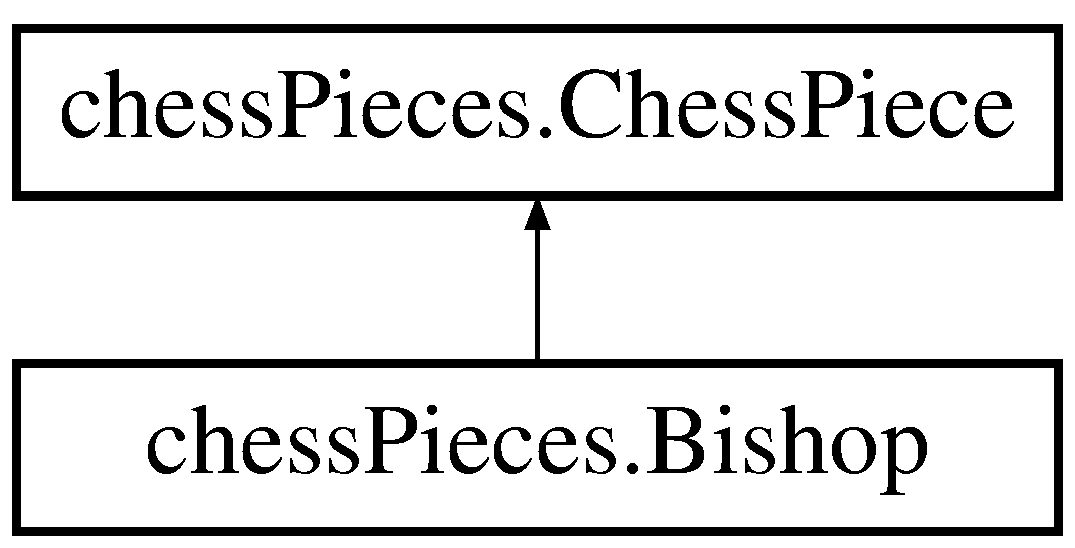
\includegraphics[height=2.000000cm]{classchess_pieces_1_1_bishop}
\end{center}
\end{figure}
\subsection*{Public Member Functions}
\begin{DoxyCompactItemize}
\item 
\hyperlink{classchess_pieces_1_1_bishop_ac939ccc917297b61fa1bc86f38bfebda}{Bishop} (String type, int number)
\item 
\hyperlink{classchess_pieces_1_1_bishop_acf607ff6a59585a2bd77f9737fa51c20}{Bishop} (String type, \hyperlink{classmodels_1_1_position}{Position} position, int number)
\item 
\hypertarget{classchess_pieces_1_1_bishop_a671e91ec066dae90ba26d390d2831892}{void {\bfseries get\+Possible\+Next\+Position} (\hyperlink{classmodels_1_1_chess_board}{Chess\+Board} chess\+Board)}\label{classchess_pieces_1_1_bishop_a671e91ec066dae90ba26d390d2831892}

\end{DoxyCompactItemize}
\subsection*{Additional Inherited Members}


\subsection{Detailed Description}
This is the class for bishop \begin{DoxyAuthor}{Author}
haoranyu 
\end{DoxyAuthor}
\begin{DoxySince}{Since}
2015-\/02-\/13 01\+:19\+:13 
\end{DoxySince}
\begin{DoxyVersion}{Version}
1.\+0 
\end{DoxyVersion}


\subsection{Constructor \& Destructor Documentation}
\hypertarget{classchess_pieces_1_1_bishop_ac939ccc917297b61fa1bc86f38bfebda}{\index{chess\+Pieces\+::\+Bishop@{chess\+Pieces\+::\+Bishop}!Bishop@{Bishop}}
\index{Bishop@{Bishop}!chess\+Pieces\+::\+Bishop@{chess\+Pieces\+::\+Bishop}}
\subsubsection[{Bishop}]{\setlength{\rightskip}{0pt plus 5cm}chess\+Pieces.\+Bishop.\+Bishop (
\begin{DoxyParamCaption}
\item[{String}]{type, }
\item[{int}]{number}
\end{DoxyParamCaption}
)}}\label{classchess_pieces_1_1_bishop_ac939ccc917297b61fa1bc86f38bfebda}
Constructor for default \hyperlink{classchess_pieces_1_1_bishop}{Bishop}


\begin{DoxyParams}{Parameters}
{\em type} & the color or null \\
\hline
{\em number} & the numbering of bishop \\
\hline
\end{DoxyParams}
\hypertarget{classchess_pieces_1_1_bishop_acf607ff6a59585a2bd77f9737fa51c20}{\index{chess\+Pieces\+::\+Bishop@{chess\+Pieces\+::\+Bishop}!Bishop@{Bishop}}
\index{Bishop@{Bishop}!chess\+Pieces\+::\+Bishop@{chess\+Pieces\+::\+Bishop}}
\subsubsection[{Bishop}]{\setlength{\rightskip}{0pt plus 5cm}chess\+Pieces.\+Bishop.\+Bishop (
\begin{DoxyParamCaption}
\item[{String}]{type, }
\item[{{\bf Position}}]{position, }
\item[{int}]{number}
\end{DoxyParamCaption}
)}}\label{classchess_pieces_1_1_bishop_acf607ff6a59585a2bd77f9737fa51c20}
Constructor for \hyperlink{classchess_pieces_1_1_bishop}{Bishop} with specified position


\begin{DoxyParams}{Parameters}
{\em type} & the color or null \\
\hline
{\em position} & the position of this bishop \\
\hline
{\em number} & the numbering of bishop \\
\hline
\end{DoxyParams}


The documentation for this class was generated from the following file\+:\begin{DoxyCompactItemize}
\item 
src/chess\+Pieces/Bishop.\+java\end{DoxyCompactItemize}

\hypertarget{classmodels_1_1_chess}{\section{models.\+Chess Class Reference}
\label{classmodels_1_1_chess}\index{models.\+Chess@{models.\+Chess}}
}
\subsection*{Static Public Member Functions}
\begin{DoxyCompactItemize}
\item 
static void \hyperlink{classmodels_1_1_chess_ad823ec16e2214b5f6a9a05988cd3b67d}{main} (String\mbox{[}$\,$\mbox{]} args)
\end{DoxyCompactItemize}


\subsection{Detailed Description}
\begin{DoxyAuthor}{Author}
haoranyu 
\end{DoxyAuthor}


\subsection{Member Function Documentation}
\hypertarget{classmodels_1_1_chess_ad823ec16e2214b5f6a9a05988cd3b67d}{\index{models\+::\+Chess@{models\+::\+Chess}!main@{main}}
\index{main@{main}!models\+::\+Chess@{models\+::\+Chess}}
\subsubsection[{main}]{\setlength{\rightskip}{0pt plus 5cm}static void models.\+Chess.\+main (
\begin{DoxyParamCaption}
\item[{String\mbox{[}$\,$\mbox{]}}]{args}
\end{DoxyParamCaption}
)\hspace{0.3cm}{\ttfamily [static]}}}\label{classmodels_1_1_chess_ad823ec16e2214b5f6a9a05988cd3b67d}

\begin{DoxyParams}{Parameters}
{\em args} & not specified \\
\hline
\end{DoxyParams}


The documentation for this class was generated from the following file\+:\begin{DoxyCompactItemize}
\item 
src/models/Chess.\+java\end{DoxyCompactItemize}

\hypertarget{classmodels_1_1_chess_board}{\section{models.\+Chess\+Board Class Reference}
\label{classmodels_1_1_chess_board}\index{models.\+Chess\+Board@{models.\+Chess\+Board}}
}
\subsection*{Public Member Functions}
\begin{DoxyCompactItemize}
\item 
\hyperlink{classmodels_1_1_chess_board_a4242ebe32dd357bd7d44b70b51eb4bf1}{Chess\+Board} ()
\item 
\hyperlink{classchess_pieces_1_1_chess_piece}{Chess\+Piece} \hyperlink{classmodels_1_1_chess_board_ab4160abcbb58f4195aa95f49263825dd}{get\+Chess\+Piece\+In\+Position} (\hyperlink{classmodels_1_1_position}{Position} position)
\item 
void \hyperlink{classmodels_1_1_chess_board_a17e3a22dfd4e07066e8751872a06b08a}{set\+Chess\+Piece\+In\+Position} (\hyperlink{classmodels_1_1_position}{Position} position, \hyperlink{classchess_pieces_1_1_chess_piece}{Chess\+Piece} chess\+Piece)
\item 
void \hyperlink{classmodels_1_1_chess_board_ab6fe2c2acb8db64021d646ffb76cc679}{clear\+Position} (\hyperlink{classmodels_1_1_position}{Position} position)
\item 
boolean \hyperlink{classmodels_1_1_chess_board_a8db97c5d6d0b15f42d7aa06054c2023f}{occupied} (\hyperlink{classmodels_1_1_position}{Position} position)
\item 
void \hyperlink{classmodels_1_1_chess_board_a0c6d29f835f288a3107103a9f33ce016}{add\+Record} (\hyperlink{classmodels_1_1_position}{Position} from\+Position, \hyperlink{classchess_pieces_1_1_chess_piece}{Chess\+Piece} from\+Chess\+Piece, \hyperlink{classmodels_1_1_position}{Position} to\+Position, \hyperlink{classchess_pieces_1_1_chess_piece}{Chess\+Piece} to\+Chess\+Piece)
\item 
\hypertarget{classmodels_1_1_chess_board_a78144a4dab1e10b9c2f75834650e224f}{\hyperlink{classmodels_1_1_record}{Record} {\bfseries last\+Record} ()}\label{classmodels_1_1_chess_board_a78144a4dab1e10b9c2f75834650e224f}

\item 
String \hyperlink{classmodels_1_1_chess_board_a7237577f7cc1880eee35f1b1ed29b762}{get\+Win} ()
\item 
void \hyperlink{classmodels_1_1_chess_board_a432547694019772c4aeee24c4e3af839}{set\+Win} (String win)
\end{DoxyCompactItemize}


\subsection{Constructor \& Destructor Documentation}
\hypertarget{classmodels_1_1_chess_board_a4242ebe32dd357bd7d44b70b51eb4bf1}{\index{models\+::\+Chess\+Board@{models\+::\+Chess\+Board}!Chess\+Board@{Chess\+Board}}
\index{Chess\+Board@{Chess\+Board}!models\+::\+Chess\+Board@{models\+::\+Chess\+Board}}
\subsubsection[{Chess\+Board}]{\setlength{\rightskip}{0pt plus 5cm}models.\+Chess\+Board.\+Chess\+Board (
\begin{DoxyParamCaption}
{}
\end{DoxyParamCaption}
)}}\label{classmodels_1_1_chess_board_a4242ebe32dd357bd7d44b70b51eb4bf1}
Constructor for a new chess\+Board with chess pieces defined 

\subsection{Member Function Documentation}
\hypertarget{classmodels_1_1_chess_board_a0c6d29f835f288a3107103a9f33ce016}{\index{models\+::\+Chess\+Board@{models\+::\+Chess\+Board}!add\+Record@{add\+Record}}
\index{add\+Record@{add\+Record}!models\+::\+Chess\+Board@{models\+::\+Chess\+Board}}
\subsubsection[{add\+Record}]{\setlength{\rightskip}{0pt plus 5cm}void models.\+Chess\+Board.\+add\+Record (
\begin{DoxyParamCaption}
\item[{{\bf Position}}]{from\+Position, }
\item[{{\bf Chess\+Piece}}]{from\+Chess\+Piece, }
\item[{{\bf Position}}]{to\+Position, }
\item[{{\bf Chess\+Piece}}]{to\+Chess\+Piece}
\end{DoxyParamCaption}
)}}\label{classmodels_1_1_chess_board_a0c6d29f835f288a3107103a9f33ce016}
A function for adding a new record 
\begin{DoxyParams}{Parameters}
{\em from\+Position} & \\
\hline
{\em from\+Chess\+Piece} & \\
\hline
{\em to\+Position} & \\
\hline
{\em to\+Chess\+Piece} & \\
\hline
\end{DoxyParams}
\hypertarget{classmodels_1_1_chess_board_ab6fe2c2acb8db64021d646ffb76cc679}{\index{models\+::\+Chess\+Board@{models\+::\+Chess\+Board}!clear\+Position@{clear\+Position}}
\index{clear\+Position@{clear\+Position}!models\+::\+Chess\+Board@{models\+::\+Chess\+Board}}
\subsubsection[{clear\+Position}]{\setlength{\rightskip}{0pt plus 5cm}void models.\+Chess\+Board.\+clear\+Position (
\begin{DoxyParamCaption}
\item[{{\bf Position}}]{position}
\end{DoxyParamCaption}
)}}\label{classmodels_1_1_chess_board_ab6fe2c2acb8db64021d646ffb76cc679}
Make the cell of position null


\begin{DoxyParams}{Parameters}
{\em position} & The position we want to clear \\
\hline
\end{DoxyParams}
\hypertarget{classmodels_1_1_chess_board_ab4160abcbb58f4195aa95f49263825dd}{\index{models\+::\+Chess\+Board@{models\+::\+Chess\+Board}!get\+Chess\+Piece\+In\+Position@{get\+Chess\+Piece\+In\+Position}}
\index{get\+Chess\+Piece\+In\+Position@{get\+Chess\+Piece\+In\+Position}!models\+::\+Chess\+Board@{models\+::\+Chess\+Board}}
\subsubsection[{get\+Chess\+Piece\+In\+Position}]{\setlength{\rightskip}{0pt plus 5cm}{\bf Chess\+Piece} models.\+Chess\+Board.\+get\+Chess\+Piece\+In\+Position (
\begin{DoxyParamCaption}
\item[{{\bf Position}}]{position}
\end{DoxyParamCaption}
)}}\label{classmodels_1_1_chess_board_ab4160abcbb58f4195aa95f49263825dd}
Get the chess\+Piece in the position


\begin{DoxyParams}{Parameters}
{\em position} & The position we see into \\
\hline
\end{DoxyParams}
\begin{DoxyReturn}{Returns}
chess\+Piece Return the chess piece in this position $\vert$ Null if not valid 
\end{DoxyReturn}
\hypertarget{classmodels_1_1_chess_board_a7237577f7cc1880eee35f1b1ed29b762}{\index{models\+::\+Chess\+Board@{models\+::\+Chess\+Board}!get\+Win@{get\+Win}}
\index{get\+Win@{get\+Win}!models\+::\+Chess\+Board@{models\+::\+Chess\+Board}}
\subsubsection[{get\+Win}]{\setlength{\rightskip}{0pt plus 5cm}String models.\+Chess\+Board.\+get\+Win (
\begin{DoxyParamCaption}
{}
\end{DoxyParamCaption}
)}}\label{classmodels_1_1_chess_board_a7237577f7cc1880eee35f1b1ed29b762}
\begin{DoxyReturn}{Returns}
the win 
\end{DoxyReturn}
\hypertarget{classmodels_1_1_chess_board_a8db97c5d6d0b15f42d7aa06054c2023f}{\index{models\+::\+Chess\+Board@{models\+::\+Chess\+Board}!occupied@{occupied}}
\index{occupied@{occupied}!models\+::\+Chess\+Board@{models\+::\+Chess\+Board}}
\subsubsection[{occupied}]{\setlength{\rightskip}{0pt plus 5cm}boolean models.\+Chess\+Board.\+occupied (
\begin{DoxyParamCaption}
\item[{{\bf Position}}]{position}
\end{DoxyParamCaption}
)}}\label{classmodels_1_1_chess_board_a8db97c5d6d0b15f42d7aa06054c2023f}
Check if the position is occupied by any chess piece


\begin{DoxyParams}{Parameters}
{\em position} & The position we see into \\
\hline
\end{DoxyParams}
\begin{DoxyReturn}{Returns}
True if any chess piece in this position 
\end{DoxyReturn}
\hypertarget{classmodels_1_1_chess_board_a17e3a22dfd4e07066e8751872a06b08a}{\index{models\+::\+Chess\+Board@{models\+::\+Chess\+Board}!set\+Chess\+Piece\+In\+Position@{set\+Chess\+Piece\+In\+Position}}
\index{set\+Chess\+Piece\+In\+Position@{set\+Chess\+Piece\+In\+Position}!models\+::\+Chess\+Board@{models\+::\+Chess\+Board}}
\subsubsection[{set\+Chess\+Piece\+In\+Position}]{\setlength{\rightskip}{0pt plus 5cm}void models.\+Chess\+Board.\+set\+Chess\+Piece\+In\+Position (
\begin{DoxyParamCaption}
\item[{{\bf Position}}]{position, }
\item[{{\bf Chess\+Piece}}]{chess\+Piece}
\end{DoxyParamCaption}
)}}\label{classmodels_1_1_chess_board_a17e3a22dfd4e07066e8751872a06b08a}
Set a chess\+Piece into the chess\+Board


\begin{DoxyParams}{Parameters}
{\em position} & The position we see into \\
\hline
{\em chess\+Piece} & The chess piece we want to put into the position \\
\hline
\end{DoxyParams}
\hypertarget{classmodels_1_1_chess_board_a432547694019772c4aeee24c4e3af839}{\index{models\+::\+Chess\+Board@{models\+::\+Chess\+Board}!set\+Win@{set\+Win}}
\index{set\+Win@{set\+Win}!models\+::\+Chess\+Board@{models\+::\+Chess\+Board}}
\subsubsection[{set\+Win}]{\setlength{\rightskip}{0pt plus 5cm}void models.\+Chess\+Board.\+set\+Win (
\begin{DoxyParamCaption}
\item[{String}]{win}
\end{DoxyParamCaption}
)}}\label{classmodels_1_1_chess_board_a432547694019772c4aeee24c4e3af839}

\begin{DoxyParams}{Parameters}
{\em win} & the win to set \\
\hline
\end{DoxyParams}


The documentation for this class was generated from the following file\+:\begin{DoxyCompactItemize}
\item 
src/models/Chess\+Board.\+java\end{DoxyCompactItemize}

\hypertarget{classchess_pieces_1_1_chess_piece}{\section{chess\+Pieces.\+Chess\+Piece Class Reference}
\label{classchess_pieces_1_1_chess_piece}\index{chess\+Pieces.\+Chess\+Piece@{chess\+Pieces.\+Chess\+Piece}}
}
Inheritance diagram for chess\+Pieces.\+Chess\+Piece\+:\begin{figure}[H]
\begin{center}
\leavevmode
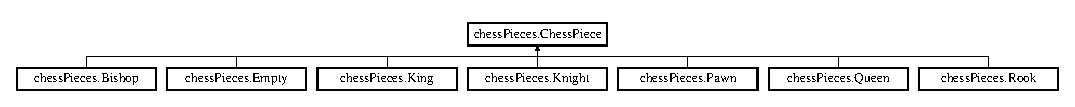
\includegraphics[height=0.987654cm]{classchess_pieces_1_1_chess_piece}
\end{center}
\end{figure}
\subsection*{Public Member Functions}
\begin{DoxyCompactItemize}
\item 
boolean \hyperlink{classchess_pieces_1_1_chess_piece_ac54942df9783962c97fc3df65e075a57}{move} (\hyperlink{classmodels_1_1_chess_board}{Chess\+Board} chess\+Board, \hyperlink{classmodels_1_1_position}{Position} new\+Position)
\item 
void \hyperlink{classchess_pieces_1_1_chess_piece_a28c442bb8fb5c8481f5ba76da5a9b95b}{show\+Possible\+Next\+Position} (\hyperlink{classmodels_1_1_chess_board}{Chess\+Board} chess\+Board)
\item 
boolean \hyperlink{classchess_pieces_1_1_chess_piece_a30832f783f609eac27f3ade1e70a67d3}{check\+Other\+King} (\hyperlink{classmodels_1_1_chess_board}{Chess\+Board} chess\+Board)
\item 
abstract void \hyperlink{classchess_pieces_1_1_chess_piece_a2286de37351ba3b330e82e6184549b01}{get\+Possible\+Next\+Position} (\hyperlink{classmodels_1_1_chess_board}{Chess\+Board} chess\+Board)
\item 
\hyperlink{classmodels_1_1_position}{Position} \hyperlink{classchess_pieces_1_1_chess_piece_a4b144240cc5b1ccec0622d72342fab99}{get\+Position} ()
\item 
void \hyperlink{classchess_pieces_1_1_chess_piece_ae365e81c758786651b7cf6fe06139177}{set\+Position} (\hyperlink{classmodels_1_1_position}{Position} position)
\item 
String \hyperlink{classchess_pieces_1_1_chess_piece_ad19f7b5dd7e7918664b90c679925d733}{get\+Type} ()
\item 
void \hyperlink{classchess_pieces_1_1_chess_piece_a8ee50123a2c6efcaf6681aa37bdf57de}{set\+Type} (String type)
\item 
String \hyperlink{classchess_pieces_1_1_chess_piece_a0e86e35efbd5d56b4377f9eba8b15569}{get\+Name} ()
\item 
void \hyperlink{classchess_pieces_1_1_chess_piece_a1a4ec57ad0f35722b789cd77bbf1f689}{set\+Name} (String name)
\end{DoxyCompactItemize}
\subsection*{Protected Member Functions}
\begin{DoxyCompactItemize}
\item 
boolean \hyperlink{classchess_pieces_1_1_chess_piece_a77b641798a0a706b4fa7a9ba9b2b99a7}{self\+Occupied} (\hyperlink{classmodels_1_1_chess_board}{Chess\+Board} chess\+Board, \hyperlink{classmodels_1_1_position}{Position} position)
\item 
boolean \hyperlink{classchess_pieces_1_1_chess_piece_ae2d53226500eae41edb706d492fe46ec}{add\+If\+Avaliable} (\hyperlink{classmodels_1_1_chess_board}{Chess\+Board} chess\+Board, \hyperlink{classmodels_1_1_position}{Position} position)
\item 
void \hyperlink{classchess_pieces_1_1_chess_piece_a584538d6c160d1b10c71979f30ec7c46}{iterative\+Add\+Possible\+Position} (\hyperlink{classmodels_1_1_chess_board}{Chess\+Board} chess\+Board, \hyperlink{classmodels_1_1_position}{Position} start\+Position, int to\+Right, int to\+Up)
\end{DoxyCompactItemize}
\subsection*{Protected Attributes}
\begin{DoxyCompactItemize}
\item 
\hypertarget{classchess_pieces_1_1_chess_piece_ab25ff9d258130b76fde382660d5b5e70}{boolean {\bfseries moved}}\label{classchess_pieces_1_1_chess_piece_ab25ff9d258130b76fde382660d5b5e70}

\item 
\hypertarget{classchess_pieces_1_1_chess_piece_acc623ade4ef4919bb496cd5d99a7019a}{String {\bfseries name}}\label{classchess_pieces_1_1_chess_piece_acc623ade4ef4919bb496cd5d99a7019a}

\item 
\hypertarget{classchess_pieces_1_1_chess_piece_a3de6dd510abf506fd4faabee948ea2fc}{String {\bfseries type}}\label{classchess_pieces_1_1_chess_piece_a3de6dd510abf506fd4faabee948ea2fc}

\item 
\hypertarget{classchess_pieces_1_1_chess_piece_a085d0f9d9a2fe2282ffa84cd32e2d2f4}{int {\bfseries number}}\label{classchess_pieces_1_1_chess_piece_a085d0f9d9a2fe2282ffa84cd32e2d2f4}

\item 
\hypertarget{classchess_pieces_1_1_chess_piece_ad2ab97750fa0e2df85710c953915588b}{\hyperlink{classmodels_1_1_position}{Position} {\bfseries position}}\label{classchess_pieces_1_1_chess_piece_ad2ab97750fa0e2df85710c953915588b}

\end{DoxyCompactItemize}


\subsection{Member Function Documentation}
\hypertarget{classchess_pieces_1_1_chess_piece_ae2d53226500eae41edb706d492fe46ec}{\index{chess\+Pieces\+::\+Chess\+Piece@{chess\+Pieces\+::\+Chess\+Piece}!add\+If\+Avaliable@{add\+If\+Avaliable}}
\index{add\+If\+Avaliable@{add\+If\+Avaliable}!chess\+Pieces\+::\+Chess\+Piece@{chess\+Pieces\+::\+Chess\+Piece}}
\subsubsection[{add\+If\+Avaliable}]{\setlength{\rightskip}{0pt plus 5cm}boolean chess\+Pieces.\+Chess\+Piece.\+add\+If\+Avaliable (
\begin{DoxyParamCaption}
\item[{{\bf Chess\+Board}}]{chess\+Board, }
\item[{{\bf Position}}]{position}
\end{DoxyParamCaption}
)\hspace{0.3cm}{\ttfamily [protected]}}}\label{classchess_pieces_1_1_chess_piece_ae2d53226500eae41edb706d492fe46ec}
If the cell is valid A\+N\+D is not self-\/occupied A\+N\+D not duplicates, Then add to possible position


\begin{DoxyParams}{Parameters}
{\em chess\+Board} & The object of chess board \\
\hline
{\em position} & The position we see into \\
\hline
\end{DoxyParams}
\begin{DoxyReturn}{Returns}
Return true if the outer iteration should going on 
\end{DoxyReturn}
\hypertarget{classchess_pieces_1_1_chess_piece_a30832f783f609eac27f3ade1e70a67d3}{\index{chess\+Pieces\+::\+Chess\+Piece@{chess\+Pieces\+::\+Chess\+Piece}!check\+Other\+King@{check\+Other\+King}}
\index{check\+Other\+King@{check\+Other\+King}!chess\+Pieces\+::\+Chess\+Piece@{chess\+Pieces\+::\+Chess\+Piece}}
\subsubsection[{check\+Other\+King}]{\setlength{\rightskip}{0pt plus 5cm}boolean chess\+Pieces.\+Chess\+Piece.\+check\+Other\+King (
\begin{DoxyParamCaption}
\item[{{\bf Chess\+Board}}]{chess\+Board}
\end{DoxyParamCaption}
)}}\label{classchess_pieces_1_1_chess_piece_a30832f783f609eac27f3ade1e70a67d3}
See whether the chess piece is now checking the other king


\begin{DoxyParams}{Parameters}
{\em chess\+Board} & The object of chess board \\
\hline
\end{DoxyParams}
\begin{DoxyReturn}{Returns}
True if there king of others is under checking 
\end{DoxyReturn}
\hypertarget{classchess_pieces_1_1_chess_piece_a0e86e35efbd5d56b4377f9eba8b15569}{\index{chess\+Pieces\+::\+Chess\+Piece@{chess\+Pieces\+::\+Chess\+Piece}!get\+Name@{get\+Name}}
\index{get\+Name@{get\+Name}!chess\+Pieces\+::\+Chess\+Piece@{chess\+Pieces\+::\+Chess\+Piece}}
\subsubsection[{get\+Name}]{\setlength{\rightskip}{0pt plus 5cm}String chess\+Pieces.\+Chess\+Piece.\+get\+Name (
\begin{DoxyParamCaption}
{}
\end{DoxyParamCaption}
)}}\label{classchess_pieces_1_1_chess_piece_a0e86e35efbd5d56b4377f9eba8b15569}
\begin{DoxyReturn}{Returns}
the name 
\end{DoxyReturn}
\hypertarget{classchess_pieces_1_1_chess_piece_a4b144240cc5b1ccec0622d72342fab99}{\index{chess\+Pieces\+::\+Chess\+Piece@{chess\+Pieces\+::\+Chess\+Piece}!get\+Position@{get\+Position}}
\index{get\+Position@{get\+Position}!chess\+Pieces\+::\+Chess\+Piece@{chess\+Pieces\+::\+Chess\+Piece}}
\subsubsection[{get\+Position}]{\setlength{\rightskip}{0pt plus 5cm}{\bf Position} chess\+Pieces.\+Chess\+Piece.\+get\+Position (
\begin{DoxyParamCaption}
{}
\end{DoxyParamCaption}
)}}\label{classchess_pieces_1_1_chess_piece_a4b144240cc5b1ccec0622d72342fab99}
\begin{DoxyReturn}{Returns}
the position 
\end{DoxyReturn}
\hypertarget{classchess_pieces_1_1_chess_piece_a2286de37351ba3b330e82e6184549b01}{\index{chess\+Pieces\+::\+Chess\+Piece@{chess\+Pieces\+::\+Chess\+Piece}!get\+Possible\+Next\+Position@{get\+Possible\+Next\+Position}}
\index{get\+Possible\+Next\+Position@{get\+Possible\+Next\+Position}!chess\+Pieces\+::\+Chess\+Piece@{chess\+Pieces\+::\+Chess\+Piece}}
\subsubsection[{get\+Possible\+Next\+Position}]{\setlength{\rightskip}{0pt plus 5cm}abstract void chess\+Pieces.\+Chess\+Piece.\+get\+Possible\+Next\+Position (
\begin{DoxyParamCaption}
\item[{{\bf Chess\+Board}}]{chess\+Board}
\end{DoxyParamCaption}
)\hspace{0.3cm}{\ttfamily [abstract]}}}\label{classchess_pieces_1_1_chess_piece_a2286de37351ba3b330e82e6184549b01}
According to the type of chess\+Piece and than calculate the possible\+Next\+Position


\begin{DoxyParams}{Parameters}
{\em chess\+Board} & The object of chess board \\
\hline
\end{DoxyParams}
\hypertarget{classchess_pieces_1_1_chess_piece_ad19f7b5dd7e7918664b90c679925d733}{\index{chess\+Pieces\+::\+Chess\+Piece@{chess\+Pieces\+::\+Chess\+Piece}!get\+Type@{get\+Type}}
\index{get\+Type@{get\+Type}!chess\+Pieces\+::\+Chess\+Piece@{chess\+Pieces\+::\+Chess\+Piece}}
\subsubsection[{get\+Type}]{\setlength{\rightskip}{0pt plus 5cm}String chess\+Pieces.\+Chess\+Piece.\+get\+Type (
\begin{DoxyParamCaption}
{}
\end{DoxyParamCaption}
)}}\label{classchess_pieces_1_1_chess_piece_ad19f7b5dd7e7918664b90c679925d733}
\begin{DoxyReturn}{Returns}
the type 
\end{DoxyReturn}
\hypertarget{classchess_pieces_1_1_chess_piece_a584538d6c160d1b10c71979f30ec7c46}{\index{chess\+Pieces\+::\+Chess\+Piece@{chess\+Pieces\+::\+Chess\+Piece}!iterative\+Add\+Possible\+Position@{iterative\+Add\+Possible\+Position}}
\index{iterative\+Add\+Possible\+Position@{iterative\+Add\+Possible\+Position}!chess\+Pieces\+::\+Chess\+Piece@{chess\+Pieces\+::\+Chess\+Piece}}
\subsubsection[{iterative\+Add\+Possible\+Position}]{\setlength{\rightskip}{0pt plus 5cm}void chess\+Pieces.\+Chess\+Piece.\+iterative\+Add\+Possible\+Position (
\begin{DoxyParamCaption}
\item[{{\bf Chess\+Board}}]{chess\+Board, }
\item[{{\bf Position}}]{start\+Position, }
\item[{int}]{to\+Right, }
\item[{int}]{to\+Up}
\end{DoxyParamCaption}
)\hspace{0.3cm}{\ttfamily [protected]}}}\label{classchess_pieces_1_1_chess_piece_a584538d6c160d1b10c71979f30ec7c46}
Iteratively checking the cells to see if available and then add


\begin{DoxyParams}{Parameters}
{\em chess\+Board} & The object of chess board \\
\hline
{\em start\+Position} & The position where iteration starts \\
\hline
{\em max\+Iteration} & The maximum iterations we are expecting \\
\hline
{\em to\+Right} & In each iteration we move how many step to right \\
\hline
{\em to\+Up} & In each iteration we move how many step to top \\
\hline
\end{DoxyParams}
\hypertarget{classchess_pieces_1_1_chess_piece_ac54942df9783962c97fc3df65e075a57}{\index{chess\+Pieces\+::\+Chess\+Piece@{chess\+Pieces\+::\+Chess\+Piece}!move@{move}}
\index{move@{move}!chess\+Pieces\+::\+Chess\+Piece@{chess\+Pieces\+::\+Chess\+Piece}}
\subsubsection[{move}]{\setlength{\rightskip}{0pt plus 5cm}boolean chess\+Pieces.\+Chess\+Piece.\+move (
\begin{DoxyParamCaption}
\item[{{\bf Chess\+Board}}]{chess\+Board, }
\item[{{\bf Position}}]{new\+Position}
\end{DoxyParamCaption}
)}}\label{classchess_pieces_1_1_chess_piece_ac54942df9783962c97fc3df65e075a57}
The move function for a chess\+Piece to move


\begin{DoxyParams}{Parameters}
{\em chess\+Board} & The object of chess board \\
\hline
{\em new\+Position} & The position we are moving to \\
\hline
\end{DoxyParams}
\begin{DoxyReturn}{Returns}
Return true if it is possible 
\end{DoxyReturn}
\hypertarget{classchess_pieces_1_1_chess_piece_a77b641798a0a706b4fa7a9ba9b2b99a7}{\index{chess\+Pieces\+::\+Chess\+Piece@{chess\+Pieces\+::\+Chess\+Piece}!self\+Occupied@{self\+Occupied}}
\index{self\+Occupied@{self\+Occupied}!chess\+Pieces\+::\+Chess\+Piece@{chess\+Pieces\+::\+Chess\+Piece}}
\subsubsection[{self\+Occupied}]{\setlength{\rightskip}{0pt plus 5cm}boolean chess\+Pieces.\+Chess\+Piece.\+self\+Occupied (
\begin{DoxyParamCaption}
\item[{{\bf Chess\+Board}}]{chess\+Board, }
\item[{{\bf Position}}]{position}
\end{DoxyParamCaption}
)\hspace{0.3cm}{\ttfamily [protected]}}}\label{classchess_pieces_1_1_chess_piece_a77b641798a0a706b4fa7a9ba9b2b99a7}
Check whether the expected position is occupied by the same color


\begin{DoxyParams}{Parameters}
{\em chess\+Board} & The object of chess board \\
\hline
{\em position} & The position we see into \\
\hline
\end{DoxyParams}
\begin{DoxyReturn}{Returns}
Return true if occupied by player himself 
\end{DoxyReturn}
\hypertarget{classchess_pieces_1_1_chess_piece_a1a4ec57ad0f35722b789cd77bbf1f689}{\index{chess\+Pieces\+::\+Chess\+Piece@{chess\+Pieces\+::\+Chess\+Piece}!set\+Name@{set\+Name}}
\index{set\+Name@{set\+Name}!chess\+Pieces\+::\+Chess\+Piece@{chess\+Pieces\+::\+Chess\+Piece}}
\subsubsection[{set\+Name}]{\setlength{\rightskip}{0pt plus 5cm}void chess\+Pieces.\+Chess\+Piece.\+set\+Name (
\begin{DoxyParamCaption}
\item[{String}]{name}
\end{DoxyParamCaption}
)}}\label{classchess_pieces_1_1_chess_piece_a1a4ec57ad0f35722b789cd77bbf1f689}

\begin{DoxyParams}{Parameters}
{\em name} & the name to set \\
\hline
\end{DoxyParams}
\hypertarget{classchess_pieces_1_1_chess_piece_ae365e81c758786651b7cf6fe06139177}{\index{chess\+Pieces\+::\+Chess\+Piece@{chess\+Pieces\+::\+Chess\+Piece}!set\+Position@{set\+Position}}
\index{set\+Position@{set\+Position}!chess\+Pieces\+::\+Chess\+Piece@{chess\+Pieces\+::\+Chess\+Piece}}
\subsubsection[{set\+Position}]{\setlength{\rightskip}{0pt plus 5cm}void chess\+Pieces.\+Chess\+Piece.\+set\+Position (
\begin{DoxyParamCaption}
\item[{{\bf Position}}]{position}
\end{DoxyParamCaption}
)}}\label{classchess_pieces_1_1_chess_piece_ae365e81c758786651b7cf6fe06139177}

\begin{DoxyParams}{Parameters}
{\em position} & the position to set \\
\hline
\end{DoxyParams}
\hypertarget{classchess_pieces_1_1_chess_piece_a8ee50123a2c6efcaf6681aa37bdf57de}{\index{chess\+Pieces\+::\+Chess\+Piece@{chess\+Pieces\+::\+Chess\+Piece}!set\+Type@{set\+Type}}
\index{set\+Type@{set\+Type}!chess\+Pieces\+::\+Chess\+Piece@{chess\+Pieces\+::\+Chess\+Piece}}
\subsubsection[{set\+Type}]{\setlength{\rightskip}{0pt plus 5cm}void chess\+Pieces.\+Chess\+Piece.\+set\+Type (
\begin{DoxyParamCaption}
\item[{String}]{type}
\end{DoxyParamCaption}
)}}\label{classchess_pieces_1_1_chess_piece_a8ee50123a2c6efcaf6681aa37bdf57de}

\begin{DoxyParams}{Parameters}
{\em type} & the type to set \\
\hline
\end{DoxyParams}
\hypertarget{classchess_pieces_1_1_chess_piece_a28c442bb8fb5c8481f5ba76da5a9b95b}{\index{chess\+Pieces\+::\+Chess\+Piece@{chess\+Pieces\+::\+Chess\+Piece}!show\+Possible\+Next\+Position@{show\+Possible\+Next\+Position}}
\index{show\+Possible\+Next\+Position@{show\+Possible\+Next\+Position}!chess\+Pieces\+::\+Chess\+Piece@{chess\+Pieces\+::\+Chess\+Piece}}
\subsubsection[{show\+Possible\+Next\+Position}]{\setlength{\rightskip}{0pt plus 5cm}void chess\+Pieces.\+Chess\+Piece.\+show\+Possible\+Next\+Position (
\begin{DoxyParamCaption}
\item[{{\bf Chess\+Board}}]{chess\+Board}
\end{DoxyParamCaption}
)}}\label{classchess_pieces_1_1_chess_piece_a28c442bb8fb5c8481f5ba76da5a9b95b}
Help function to show all possible function W\+I\+L\+L B\+E R\+E\+M\+O\+V\+E\+D L\+A\+T\+E\+R


\begin{DoxyParams}{Parameters}
{\em chess\+Board} & The object of chess board \\
\hline
\end{DoxyParams}


The documentation for this class was generated from the following file\+:\begin{DoxyCompactItemize}
\item 
src/chess\+Pieces/Chess\+Piece.\+java\end{DoxyCompactItemize}

\hypertarget{classchess_pieces_1_1_empty}{\section{chess\+Pieces.\+Empty Class Reference}
\label{classchess_pieces_1_1_empty}\index{chess\+Pieces.\+Empty@{chess\+Pieces.\+Empty}}
}
Inheritance diagram for chess\+Pieces.\+Empty\+:\begin{figure}[H]
\begin{center}
\leavevmode
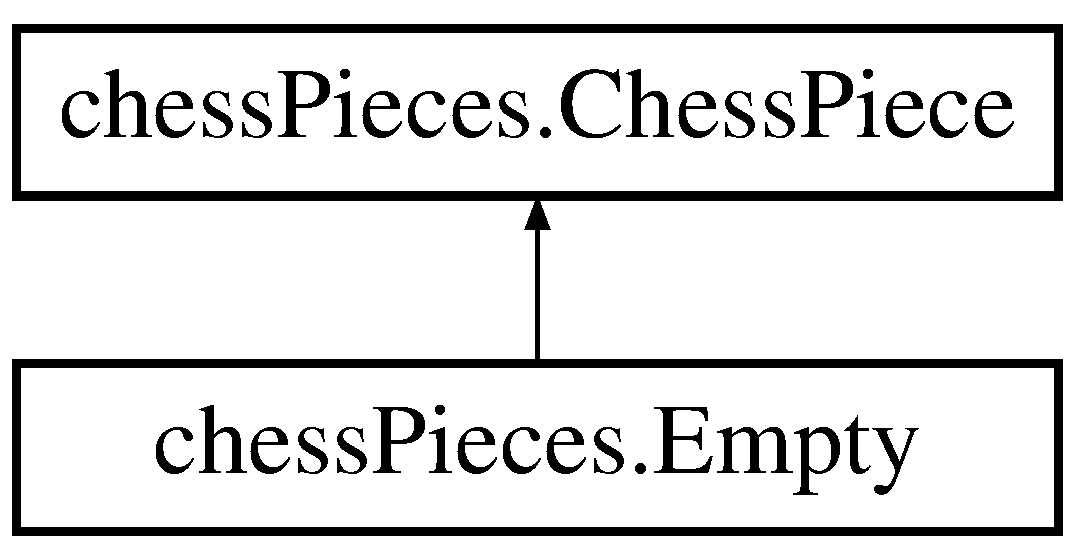
\includegraphics[height=2.000000cm]{classchess_pieces_1_1_empty}
\end{center}
\end{figure}
\subsection*{Public Member Functions}
\begin{DoxyCompactItemize}
\item 
\hypertarget{classchess_pieces_1_1_empty_ab8318f2c170f9957bfedc33d27c27868}{void {\bfseries get\+Possible\+Next\+Position} (\hyperlink{classmodels_1_1_chess_board}{Chess\+Board} chess\+Board)}\label{classchess_pieces_1_1_empty_ab8318f2c170f9957bfedc33d27c27868}

\end{DoxyCompactItemize}
\subsection*{Additional Inherited Members}


\subsection{Detailed Description}
This is the class for no chess piece (a special chess piece called \hyperlink{classchess_pieces_1_1_empty}{Empty}) Any empty cell in the chess board will be viewed as empty chess piece. \begin{DoxyAuthor}{Author}
haoranyu 
\end{DoxyAuthor}
\begin{DoxySince}{Since}
2015-\/02-\/13 01\+:19\+:17 
\end{DoxySince}
\begin{DoxyVersion}{Version}
1.\+0 
\end{DoxyVersion}


The documentation for this class was generated from the following file\+:\begin{DoxyCompactItemize}
\item 
src/chess\+Pieces/Empty.\+java\end{DoxyCompactItemize}

\hypertarget{classchess_pieces_1_1_king}{\section{chess\+Pieces.\+King Class Reference}
\label{classchess_pieces_1_1_king}\index{chess\+Pieces.\+King@{chess\+Pieces.\+King}}
}
Inheritance diagram for chess\+Pieces.\+King\+:\begin{figure}[H]
\begin{center}
\leavevmode
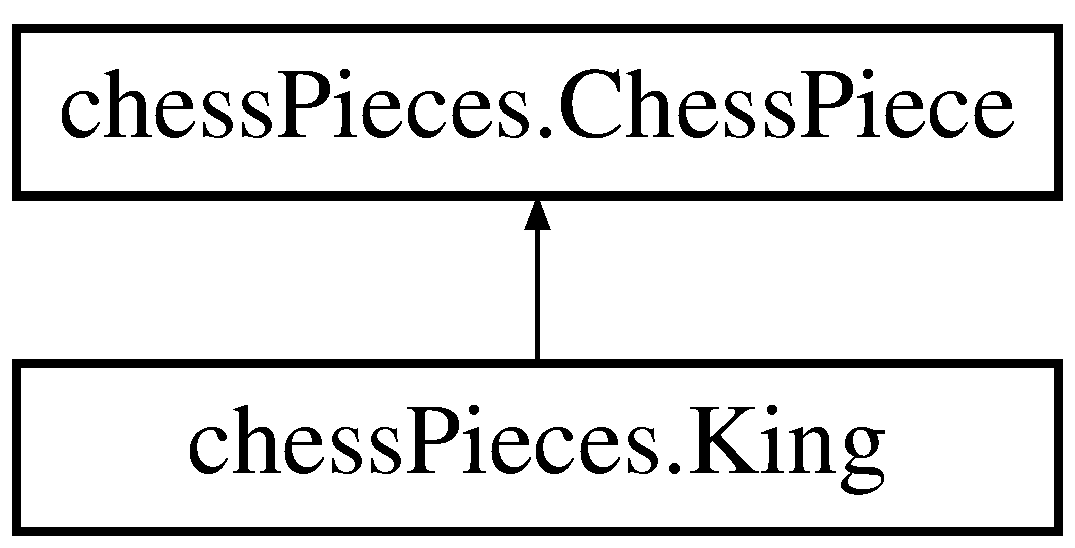
\includegraphics[height=2.000000cm]{classchess_pieces_1_1_king}
\end{center}
\end{figure}
\subsection*{Public Member Functions}
\begin{DoxyCompactItemize}
\item 
\hyperlink{classchess_pieces_1_1_king_a66cabcc1ead5022216f5ed170a4c4bd6}{King} (String type)
\item 
\hyperlink{classchess_pieces_1_1_king_a7a84e3a42cf0ea6b242383381ceee51b}{King} (String type, \hyperlink{classmodels_1_1_position}{Position} position)
\item 
\hypertarget{classchess_pieces_1_1_king_a8dad37f9c467f85dbcbe893726f67078}{void {\bfseries get\+Possible\+Next\+Position} (\hyperlink{classmodels_1_1_chess_board}{Chess\+Board} chess\+Board)}\label{classchess_pieces_1_1_king_a8dad37f9c467f85dbcbe893726f67078}

\end{DoxyCompactItemize}
\subsection*{Additional Inherited Members}


\subsection{Detailed Description}
This is the class for king \begin{DoxyAuthor}{Author}
haoranyu 
\end{DoxyAuthor}
\begin{DoxySince}{Since}
2015-\/02-\/13 01\+:19\+:22 
\end{DoxySince}
\begin{DoxyVersion}{Version}
1.\+0 
\end{DoxyVersion}


\subsection{Constructor \& Destructor Documentation}
\hypertarget{classchess_pieces_1_1_king_a66cabcc1ead5022216f5ed170a4c4bd6}{\index{chess\+Pieces\+::\+King@{chess\+Pieces\+::\+King}!King@{King}}
\index{King@{King}!chess\+Pieces\+::\+King@{chess\+Pieces\+::\+King}}
\subsubsection[{King}]{\setlength{\rightskip}{0pt plus 5cm}chess\+Pieces.\+King.\+King (
\begin{DoxyParamCaption}
\item[{String}]{type}
\end{DoxyParamCaption}
)}}\label{classchess_pieces_1_1_king_a66cabcc1ead5022216f5ed170a4c4bd6}
Constructor for default \hyperlink{classchess_pieces_1_1_king}{King}


\begin{DoxyParams}{Parameters}
{\em type} & the color or null \\
\hline
\end{DoxyParams}
\hypertarget{classchess_pieces_1_1_king_a7a84e3a42cf0ea6b242383381ceee51b}{\index{chess\+Pieces\+::\+King@{chess\+Pieces\+::\+King}!King@{King}}
\index{King@{King}!chess\+Pieces\+::\+King@{chess\+Pieces\+::\+King}}
\subsubsection[{King}]{\setlength{\rightskip}{0pt plus 5cm}chess\+Pieces.\+King.\+King (
\begin{DoxyParamCaption}
\item[{String}]{type, }
\item[{{\bf Position}}]{position}
\end{DoxyParamCaption}
)}}\label{classchess_pieces_1_1_king_a7a84e3a42cf0ea6b242383381ceee51b}
Constructor for \hyperlink{classchess_pieces_1_1_king}{King} with specified position


\begin{DoxyParams}{Parameters}
{\em type} & the color or null \\
\hline
{\em position} & the position of this king \\
\hline
\end{DoxyParams}


The documentation for this class was generated from the following file\+:\begin{DoxyCompactItemize}
\item 
src/chess\+Pieces/King.\+java\end{DoxyCompactItemize}

\hypertarget{classchess_pieces_1_1_knight}{\section{chess\+Pieces.\+Knight Class Reference}
\label{classchess_pieces_1_1_knight}\index{chess\+Pieces.\+Knight@{chess\+Pieces.\+Knight}}
}
Inheritance diagram for chess\+Pieces.\+Knight\+:\begin{figure}[H]
\begin{center}
\leavevmode
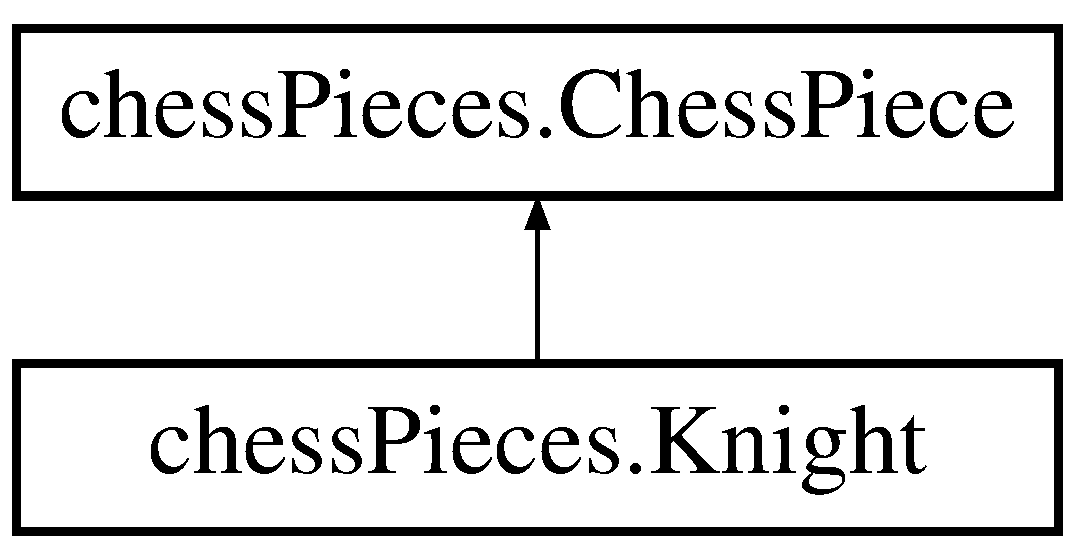
\includegraphics[height=2.000000cm]{classchess_pieces_1_1_knight}
\end{center}
\end{figure}
\subsection*{Public Member Functions}
\begin{DoxyCompactItemize}
\item 
\hyperlink{classchess_pieces_1_1_knight_aca1a0fe4a874da1aa6ebfa21afa9a6fc}{Knight} (String type, int number)
\item 
\hyperlink{classchess_pieces_1_1_knight_a60358d795fb1c3ea5288b31df4388096}{Knight} (String type, \hyperlink{classmodels_1_1_position}{Position} position, int number)
\item 
\hypertarget{classchess_pieces_1_1_knight_a41d69df8de591fe6717fb524ff0fcf42}{void {\bfseries get\+Possible\+Next\+Position} (\hyperlink{classmodels_1_1_chess_board}{Chess\+Board} chess\+Board)}\label{classchess_pieces_1_1_knight_a41d69df8de591fe6717fb524ff0fcf42}

\end{DoxyCompactItemize}
\subsection*{Additional Inherited Members}


\subsection{Detailed Description}
This is the class for knight \begin{DoxyAuthor}{Author}
haoranyu 
\end{DoxyAuthor}
\begin{DoxySince}{Since}
2015-\/02-\/13 01\+:19\+:26 
\end{DoxySince}
\begin{DoxyVersion}{Version}
1.\+0 
\end{DoxyVersion}


\subsection{Constructor \& Destructor Documentation}
\hypertarget{classchess_pieces_1_1_knight_aca1a0fe4a874da1aa6ebfa21afa9a6fc}{\index{chess\+Pieces\+::\+Knight@{chess\+Pieces\+::\+Knight}!Knight@{Knight}}
\index{Knight@{Knight}!chess\+Pieces\+::\+Knight@{chess\+Pieces\+::\+Knight}}
\subsubsection[{Knight}]{\setlength{\rightskip}{0pt plus 5cm}chess\+Pieces.\+Knight.\+Knight (
\begin{DoxyParamCaption}
\item[{String}]{type, }
\item[{int}]{number}
\end{DoxyParamCaption}
)}}\label{classchess_pieces_1_1_knight_aca1a0fe4a874da1aa6ebfa21afa9a6fc}
Constructor for default \hyperlink{classchess_pieces_1_1_knight}{Knight}


\begin{DoxyParams}{Parameters}
{\em type} & the color or null \\
\hline
{\em number} & the numbering of knight \\
\hline
\end{DoxyParams}
\hypertarget{classchess_pieces_1_1_knight_a60358d795fb1c3ea5288b31df4388096}{\index{chess\+Pieces\+::\+Knight@{chess\+Pieces\+::\+Knight}!Knight@{Knight}}
\index{Knight@{Knight}!chess\+Pieces\+::\+Knight@{chess\+Pieces\+::\+Knight}}
\subsubsection[{Knight}]{\setlength{\rightskip}{0pt plus 5cm}chess\+Pieces.\+Knight.\+Knight (
\begin{DoxyParamCaption}
\item[{String}]{type, }
\item[{{\bf Position}}]{position, }
\item[{int}]{number}
\end{DoxyParamCaption}
)}}\label{classchess_pieces_1_1_knight_a60358d795fb1c3ea5288b31df4388096}
Constructor for \hyperlink{classchess_pieces_1_1_knight}{Knight} with specified position


\begin{DoxyParams}{Parameters}
{\em type} & the color or null \\
\hline
{\em position} & the position of this knight \\
\hline
{\em number} & the numbering of knight \\
\hline
\end{DoxyParams}


The documentation for this class was generated from the following file\+:\begin{DoxyCompactItemize}
\item 
src/chess\+Pieces/Knight.\+java\end{DoxyCompactItemize}

\hypertarget{classchess_pieces_1_1_pawn}{\section{chess\+Pieces.\+Pawn Class Reference}
\label{classchess_pieces_1_1_pawn}\index{chess\+Pieces.\+Pawn@{chess\+Pieces.\+Pawn}}
}
Inheritance diagram for chess\+Pieces.\+Pawn\+:\begin{figure}[H]
\begin{center}
\leavevmode
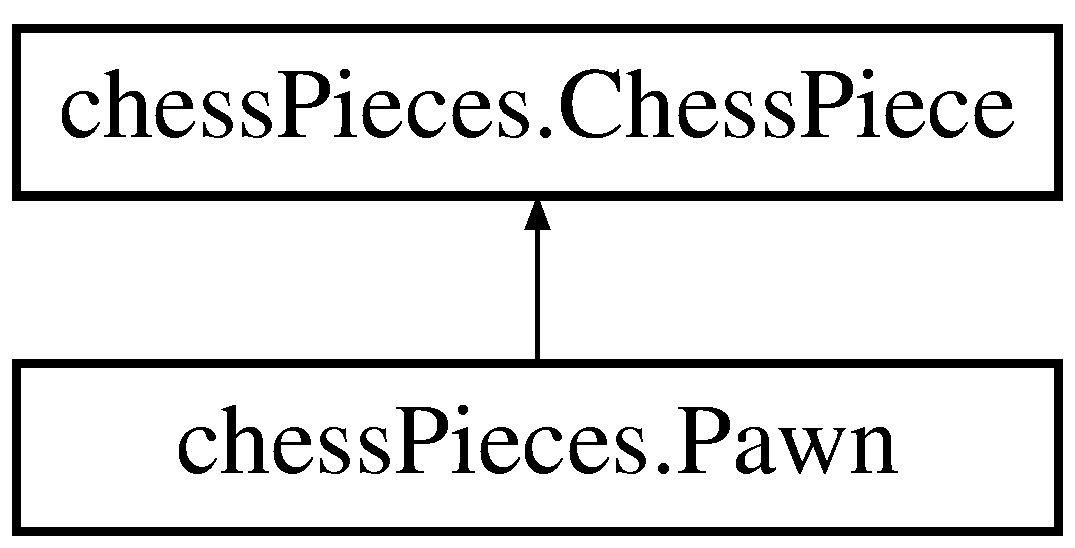
\includegraphics[height=2.000000cm]{classchess_pieces_1_1_pawn}
\end{center}
\end{figure}
\subsection*{Public Member Functions}
\begin{DoxyCompactItemize}
\item 
\hyperlink{classchess_pieces_1_1_pawn_a7cb5f02c0e0dd7707d4d3abdf7161c84}{Pawn} (String type, int number)
\item 
\hyperlink{classchess_pieces_1_1_pawn_a2c4bdb4c195fbd53e4cea91dd4cab53c}{Pawn} (String type, \hyperlink{classmodels_1_1_position}{Position} position, int number)
\item 
\hypertarget{classchess_pieces_1_1_pawn_acbb0a17aaac9f15f5e7d33c94e9f47ed}{void {\bfseries get\+Possible\+Next\+Position} (\hyperlink{classmodels_1_1_chess_board}{Chess\+Board} chess\+Board)}\label{classchess_pieces_1_1_pawn_acbb0a17aaac9f15f5e7d33c94e9f47ed}

\end{DoxyCompactItemize}
\subsection*{Protected Member Functions}
\begin{DoxyCompactItemize}
\item 
boolean \hyperlink{classchess_pieces_1_1_pawn_a5788751e93b88159665f3533b3b5b311}{add\+If\+Avaliable} (\hyperlink{classmodels_1_1_chess_board}{Chess\+Board} chess\+Board, \hyperlink{classmodels_1_1_position}{Position} position)
\end{DoxyCompactItemize}
\subsection*{Additional Inherited Members}


\subsection{Detailed Description}
This is the class for pawn \begin{DoxyAuthor}{Author}
haoranyu 
\end{DoxyAuthor}
\begin{DoxySince}{Since}
2015-\/02-\/13 16\+:48\+:36 
\end{DoxySince}
\begin{DoxyVersion}{Version}
1.\+0 
\end{DoxyVersion}


\subsection{Constructor \& Destructor Documentation}
\hypertarget{classchess_pieces_1_1_pawn_a7cb5f02c0e0dd7707d4d3abdf7161c84}{\index{chess\+Pieces\+::\+Pawn@{chess\+Pieces\+::\+Pawn}!Pawn@{Pawn}}
\index{Pawn@{Pawn}!chess\+Pieces\+::\+Pawn@{chess\+Pieces\+::\+Pawn}}
\subsubsection[{Pawn}]{\setlength{\rightskip}{0pt plus 5cm}chess\+Pieces.\+Pawn.\+Pawn (
\begin{DoxyParamCaption}
\item[{String}]{type, }
\item[{int}]{number}
\end{DoxyParamCaption}
)}}\label{classchess_pieces_1_1_pawn_a7cb5f02c0e0dd7707d4d3abdf7161c84}
Constructor for default \hyperlink{classchess_pieces_1_1_pawn}{Pawn}


\begin{DoxyParams}{Parameters}
{\em type} & the color or null \\
\hline
{\em number} & the numbering of pawn \\
\hline
\end{DoxyParams}
\hypertarget{classchess_pieces_1_1_pawn_a2c4bdb4c195fbd53e4cea91dd4cab53c}{\index{chess\+Pieces\+::\+Pawn@{chess\+Pieces\+::\+Pawn}!Pawn@{Pawn}}
\index{Pawn@{Pawn}!chess\+Pieces\+::\+Pawn@{chess\+Pieces\+::\+Pawn}}
\subsubsection[{Pawn}]{\setlength{\rightskip}{0pt plus 5cm}chess\+Pieces.\+Pawn.\+Pawn (
\begin{DoxyParamCaption}
\item[{String}]{type, }
\item[{{\bf Position}}]{position, }
\item[{int}]{number}
\end{DoxyParamCaption}
)}}\label{classchess_pieces_1_1_pawn_a2c4bdb4c195fbd53e4cea91dd4cab53c}
Constructor for \hyperlink{classchess_pieces_1_1_pawn}{Pawn} with specified position


\begin{DoxyParams}{Parameters}
{\em type} & the color or null \\
\hline
{\em position} & the position of this pawn \\
\hline
{\em number} & the numbering of pawn \\
\hline
\end{DoxyParams}


\subsection{Member Function Documentation}
\hypertarget{classchess_pieces_1_1_pawn_a5788751e93b88159665f3533b3b5b311}{\index{chess\+Pieces\+::\+Pawn@{chess\+Pieces\+::\+Pawn}!add\+If\+Avaliable@{add\+If\+Avaliable}}
\index{add\+If\+Avaliable@{add\+If\+Avaliable}!chess\+Pieces\+::\+Pawn@{chess\+Pieces\+::\+Pawn}}
\subsubsection[{add\+If\+Avaliable}]{\setlength{\rightskip}{0pt plus 5cm}boolean chess\+Pieces.\+Pawn.\+add\+If\+Avaliable (
\begin{DoxyParamCaption}
\item[{{\bf Chess\+Board}}]{chess\+Board, }
\item[{{\bf Position}}]{position}
\end{DoxyParamCaption}
)\hspace{0.3cm}{\ttfamily [protected]}}}\label{classchess_pieces_1_1_pawn_a5788751e93b88159665f3533b3b5b311}
This override for \hyperlink{classchess_pieces_1_1_pawn}{Pawn} case which is special If the cell is valid A\+N\+D is not self-\/occupied A\+N\+D not duplicates, Then add to possible position


\begin{DoxyParams}{Parameters}
{\em chess\+Board} & The object of chess board \\
\hline
{\em position} & The position we see into \\
\hline
\end{DoxyParams}


The documentation for this class was generated from the following file\+:\begin{DoxyCompactItemize}
\item 
src/chess\+Pieces/Pawn.\+java\end{DoxyCompactItemize}

\hypertarget{classmodels_1_1_position}{\section{models.\+Position Class Reference}
\label{classmodels_1_1_position}\index{models.\+Position@{models.\+Position}}
}
\subsection*{Public Member Functions}
\begin{DoxyCompactItemize}
\item 
\hyperlink{classmodels_1_1_position_ae70489b2d6b4738da8a2018e61634a6d}{Position} ()
\item 
\hyperlink{classmodels_1_1_position_ac71bfa61225c295e8554e9f22858e105}{Position} (\hyperlink{classmodels_1_1_position}{Position} position)
\item 
\hyperlink{classmodels_1_1_position_a3ca0f8a082cd6da56549403397facdbf}{Position} (int row, int col)
\item 
\hyperlink{classmodels_1_1_position}{Position} \hyperlink{classmodels_1_1_position_a15c414693b69ee5685697faa77b35247}{get\+Right} (int step)
\item 
\hyperlink{classmodels_1_1_position}{Position} \hyperlink{classmodels_1_1_position_af6beee2dd50788597e1ee1a44854bdd7}{get\+Left} (int step)
\item 
\hyperlink{classmodels_1_1_position}{Position} \hyperlink{classmodels_1_1_position_af2c7aeae4f0c5cf9d9c752020fada35a}{get\+Up} (int step)
\item 
\hyperlink{classmodels_1_1_position}{Position} \hyperlink{classmodels_1_1_position_a5edb65a1f0e1e83b116ec155315da33a}{get\+Down} (int step)
\item 
void \hyperlink{classmodels_1_1_position_ad0778a05537f93acd82e31a6d053e380}{show} ()
\item 
boolean \hyperlink{classmodels_1_1_position_af999cad6749ec695abed16c2f4404370}{valid} (\hyperlink{classmodels_1_1_chess_board}{Chess\+Board} chess\+Board)
\item 
boolean \hyperlink{classmodels_1_1_position_a25c38e3b3fbdf544b88dc328aceb0aad}{equals} (Object object)
\item 
int \hyperlink{classmodels_1_1_position_ae8e5288bb6a72118ef901adb7e70e756}{hash\+Code} ()
\item 
int \hyperlink{classmodels_1_1_position_ae3739c95264be83590bdd5cc8800f5c3}{get\+Col} ()
\end{DoxyCompactItemize}


\subsection{Detailed Description}
This is the class for position on the chess board \begin{DoxyAuthor}{Author}
haoranyu 
\end{DoxyAuthor}
\begin{DoxySince}{Since}
2015-\/02-\/13 01\+:19\+:47 
\end{DoxySince}
\begin{DoxyVersion}{Version}
1.\+0 
\end{DoxyVersion}


\subsection{Constructor \& Destructor Documentation}
\hypertarget{classmodels_1_1_position_ae70489b2d6b4738da8a2018e61634a6d}{\index{models\+::\+Position@{models\+::\+Position}!Position@{Position}}
\index{Position@{Position}!models\+::\+Position@{models\+::\+Position}}
\subsubsection[{Position}]{\setlength{\rightskip}{0pt plus 5cm}models.\+Position.\+Position (
\begin{DoxyParamCaption}
{}
\end{DoxyParamCaption}
)}}\label{classmodels_1_1_position_ae70489b2d6b4738da8a2018e61634a6d}
Constructor with no parameters Get a position without meaning \hypertarget{classmodels_1_1_position_ac71bfa61225c295e8554e9f22858e105}{\index{models\+::\+Position@{models\+::\+Position}!Position@{Position}}
\index{Position@{Position}!models\+::\+Position@{models\+::\+Position}}
\subsubsection[{Position}]{\setlength{\rightskip}{0pt plus 5cm}models.\+Position.\+Position (
\begin{DoxyParamCaption}
\item[{{\bf Position}}]{position}
\end{DoxyParamCaption}
)}}\label{classmodels_1_1_position_ac71bfa61225c295e8554e9f22858e105}
Copy constructor


\begin{DoxyParams}{Parameters}
{\em position} & The position to copy from \\
\hline
\end{DoxyParams}
\hypertarget{classmodels_1_1_position_a3ca0f8a082cd6da56549403397facdbf}{\index{models\+::\+Position@{models\+::\+Position}!Position@{Position}}
\index{Position@{Position}!models\+::\+Position@{models\+::\+Position}}
\subsubsection[{Position}]{\setlength{\rightskip}{0pt plus 5cm}models.\+Position.\+Position (
\begin{DoxyParamCaption}
\item[{int}]{row, }
\item[{int}]{col}
\end{DoxyParamCaption}
)}}\label{classmodels_1_1_position_a3ca0f8a082cd6da56549403397facdbf}
Constructor of \hyperlink{classmodels_1_1_position}{Position} with initial row and column


\begin{DoxyParams}{Parameters}
{\em row} & The row of position to initialize from \\
\hline
{\em col} & The column of position to initialize from \\
\hline
\end{DoxyParams}


\subsection{Member Function Documentation}
\hypertarget{classmodels_1_1_position_a25c38e3b3fbdf544b88dc328aceb0aad}{\index{models\+::\+Position@{models\+::\+Position}!equals@{equals}}
\index{equals@{equals}!models\+::\+Position@{models\+::\+Position}}
\subsubsection[{equals}]{\setlength{\rightskip}{0pt plus 5cm}boolean models.\+Position.\+equals (
\begin{DoxyParamCaption}
\item[{Object}]{object}
\end{DoxyParamCaption}
)}}\label{classmodels_1_1_position_a25c38e3b3fbdf544b88dc328aceb0aad}
Override original equals function

\begin{DoxySeeAlso}{See also}
java.\+lang.\+Object\+::equals(java.\+lang.\+Object) 
\end{DoxySeeAlso}
\hypertarget{classmodels_1_1_position_ae3739c95264be83590bdd5cc8800f5c3}{\index{models\+::\+Position@{models\+::\+Position}!get\+Col@{get\+Col}}
\index{get\+Col@{get\+Col}!models\+::\+Position@{models\+::\+Position}}
\subsubsection[{get\+Col}]{\setlength{\rightskip}{0pt plus 5cm}int models.\+Position.\+get\+Col (
\begin{DoxyParamCaption}
{}
\end{DoxyParamCaption}
)}}\label{classmodels_1_1_position_ae3739c95264be83590bdd5cc8800f5c3}
\begin{DoxyReturn}{Returns}
the col 
\end{DoxyReturn}
\hypertarget{classmodels_1_1_position_a5edb65a1f0e1e83b116ec155315da33a}{\index{models\+::\+Position@{models\+::\+Position}!get\+Down@{get\+Down}}
\index{get\+Down@{get\+Down}!models\+::\+Position@{models\+::\+Position}}
\subsubsection[{get\+Down}]{\setlength{\rightskip}{0pt plus 5cm}{\bf Position} models.\+Position.\+get\+Down (
\begin{DoxyParamCaption}
\item[{int}]{step}
\end{DoxyParamCaption}
)}}\label{classmodels_1_1_position_a5edb65a1f0e1e83b116ec155315da33a}
Get the position to \#step away to the bottom


\begin{DoxyParams}{Parameters}
{\em step} & The number of steps \\
\hline
\end{DoxyParams}
\begin{DoxyReturn}{Returns}
The new position after calucation 
\end{DoxyReturn}
\hypertarget{classmodels_1_1_position_af6beee2dd50788597e1ee1a44854bdd7}{\index{models\+::\+Position@{models\+::\+Position}!get\+Left@{get\+Left}}
\index{get\+Left@{get\+Left}!models\+::\+Position@{models\+::\+Position}}
\subsubsection[{get\+Left}]{\setlength{\rightskip}{0pt plus 5cm}{\bf Position} models.\+Position.\+get\+Left (
\begin{DoxyParamCaption}
\item[{int}]{step}
\end{DoxyParamCaption}
)}}\label{classmodels_1_1_position_af6beee2dd50788597e1ee1a44854bdd7}
Get the position to \#step away to the left


\begin{DoxyParams}{Parameters}
{\em step} & The number of steps \\
\hline
\end{DoxyParams}
\begin{DoxyReturn}{Returns}
The new position after calucation 
\end{DoxyReturn}
\hypertarget{classmodels_1_1_position_a15c414693b69ee5685697faa77b35247}{\index{models\+::\+Position@{models\+::\+Position}!get\+Right@{get\+Right}}
\index{get\+Right@{get\+Right}!models\+::\+Position@{models\+::\+Position}}
\subsubsection[{get\+Right}]{\setlength{\rightskip}{0pt plus 5cm}{\bf Position} models.\+Position.\+get\+Right (
\begin{DoxyParamCaption}
\item[{int}]{step}
\end{DoxyParamCaption}
)}}\label{classmodels_1_1_position_a15c414693b69ee5685697faa77b35247}
Get the position to \#step away to the right


\begin{DoxyParams}{Parameters}
{\em step} & The number of steps \\
\hline
\end{DoxyParams}
\begin{DoxyReturn}{Returns}
The new position after calucation 
\end{DoxyReturn}
\hypertarget{classmodels_1_1_position_af2c7aeae4f0c5cf9d9c752020fada35a}{\index{models\+::\+Position@{models\+::\+Position}!get\+Up@{get\+Up}}
\index{get\+Up@{get\+Up}!models\+::\+Position@{models\+::\+Position}}
\subsubsection[{get\+Up}]{\setlength{\rightskip}{0pt plus 5cm}{\bf Position} models.\+Position.\+get\+Up (
\begin{DoxyParamCaption}
\item[{int}]{step}
\end{DoxyParamCaption}
)}}\label{classmodels_1_1_position_af2c7aeae4f0c5cf9d9c752020fada35a}
Get the position to \#step away to the top


\begin{DoxyParams}{Parameters}
{\em step} & The number of steps \\
\hline
\end{DoxyParams}
\begin{DoxyReturn}{Returns}
The new position after calucation 
\end{DoxyReturn}
\hypertarget{classmodels_1_1_position_ae8e5288bb6a72118ef901adb7e70e756}{\index{models\+::\+Position@{models\+::\+Position}!hash\+Code@{hash\+Code}}
\index{hash\+Code@{hash\+Code}!models\+::\+Position@{models\+::\+Position}}
\subsubsection[{hash\+Code}]{\setlength{\rightskip}{0pt plus 5cm}int models.\+Position.\+hash\+Code (
\begin{DoxyParamCaption}
{}
\end{DoxyParamCaption}
)}}\label{classmodels_1_1_position_ae8e5288bb6a72118ef901adb7e70e756}
Override original hash\+Code function

\begin{DoxySeeAlso}{See also}
java.\+lang.\+Object\+::hash\+Code() 
\end{DoxySeeAlso}
\hypertarget{classmodels_1_1_position_ad0778a05537f93acd82e31a6d053e380}{\index{models\+::\+Position@{models\+::\+Position}!show@{show}}
\index{show@{show}!models\+::\+Position@{models\+::\+Position}}
\subsubsection[{show}]{\setlength{\rightskip}{0pt plus 5cm}void models.\+Position.\+show (
\begin{DoxyParamCaption}
{}
\end{DoxyParamCaption}
)}}\label{classmodels_1_1_position_ad0778a05537f93acd82e31a6d053e380}
A print out help function that print the pair of position W\+I\+L\+L B\+E R\+E\+M\+O\+V\+E\+D L\+A\+T\+E\+R \hypertarget{classmodels_1_1_position_af999cad6749ec695abed16c2f4404370}{\index{models\+::\+Position@{models\+::\+Position}!valid@{valid}}
\index{valid@{valid}!models\+::\+Position@{models\+::\+Position}}
\subsubsection[{valid}]{\setlength{\rightskip}{0pt plus 5cm}boolean models.\+Position.\+valid (
\begin{DoxyParamCaption}
\item[{{\bf Chess\+Board}}]{chess\+Board}
\end{DoxyParamCaption}
)}}\label{classmodels_1_1_position_af999cad6749ec695abed16c2f4404370}
Test whether the position is in the chess board


\begin{DoxyParams}{Parameters}
{\em chess\+Board} & The chess board we see into \\
\hline
\end{DoxyParams}
\begin{DoxyReturn}{Returns}
True if the row and column specified exist in the chess board 
\end{DoxyReturn}


The documentation for this class was generated from the following file\+:\begin{DoxyCompactItemize}
\item 
src/models/Position.\+java\end{DoxyCompactItemize}

\hypertarget{classchess_pieces_1_1_queen}{\section{chess\+Pieces.\+Queen Class Reference}
\label{classchess_pieces_1_1_queen}\index{chess\+Pieces.\+Queen@{chess\+Pieces.\+Queen}}
}
Inheritance diagram for chess\+Pieces.\+Queen\+:\begin{figure}[H]
\begin{center}
\leavevmode
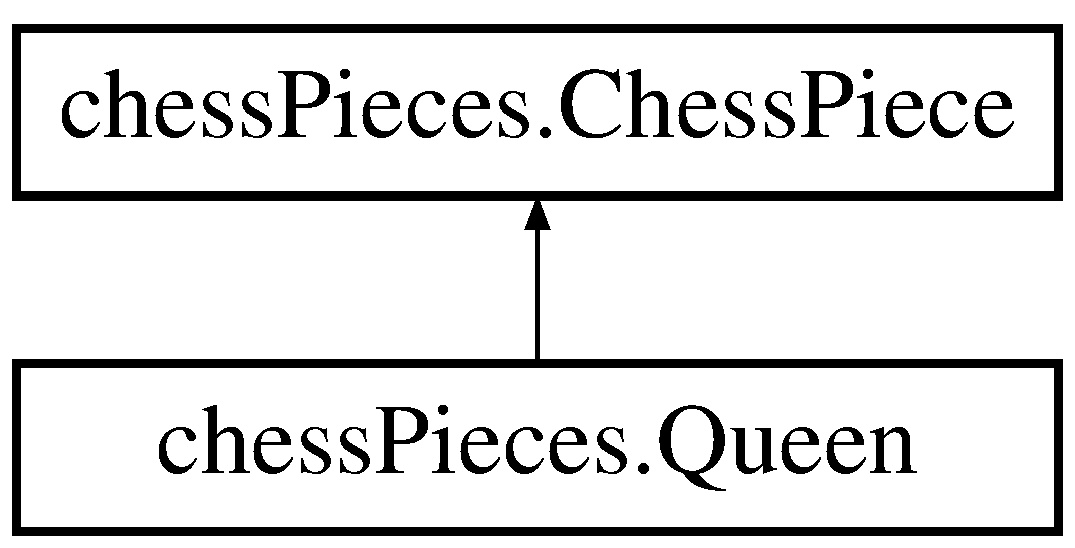
\includegraphics[height=2.000000cm]{classchess_pieces_1_1_queen}
\end{center}
\end{figure}
\subsection*{Public Member Functions}
\begin{DoxyCompactItemize}
\item 
\hyperlink{classchess_pieces_1_1_queen_a72bb7eddfbc1b52ccb3869454cacf631}{Queen} (String type)
\item 
\hyperlink{classchess_pieces_1_1_queen_a722ac44808afa09a2a381c17dd27d363}{Queen} (String type, \hyperlink{classmodels_1_1_position}{Position} position)
\item 
\hypertarget{classchess_pieces_1_1_queen_a3b76122829ccf1bee5f1cacbdbc6ae95}{void {\bfseries get\+Possible\+Next\+Position} (\hyperlink{classmodels_1_1_chess_board}{Chess\+Board} chess\+Board)}\label{classchess_pieces_1_1_queen_a3b76122829ccf1bee5f1cacbdbc6ae95}

\end{DoxyCompactItemize}
\subsection*{Additional Inherited Members}


\subsection{Detailed Description}
This is the class for queen \begin{DoxyAuthor}{Author}
haoranyu 
\end{DoxyAuthor}
\begin{DoxySince}{Since}
2015-\/02-\/13 01\+:19\+:38 
\end{DoxySince}
\begin{DoxyVersion}{Version}
1.\+0 
\end{DoxyVersion}


\subsection{Constructor \& Destructor Documentation}
\hypertarget{classchess_pieces_1_1_queen_a72bb7eddfbc1b52ccb3869454cacf631}{\index{chess\+Pieces\+::\+Queen@{chess\+Pieces\+::\+Queen}!Queen@{Queen}}
\index{Queen@{Queen}!chess\+Pieces\+::\+Queen@{chess\+Pieces\+::\+Queen}}
\subsubsection[{Queen}]{\setlength{\rightskip}{0pt plus 5cm}chess\+Pieces.\+Queen.\+Queen (
\begin{DoxyParamCaption}
\item[{String}]{type}
\end{DoxyParamCaption}
)}}\label{classchess_pieces_1_1_queen_a72bb7eddfbc1b52ccb3869454cacf631}
Constructor for default \hyperlink{classchess_pieces_1_1_queen}{Queen}


\begin{DoxyParams}{Parameters}
{\em type} & the color or null \\
\hline
\end{DoxyParams}
\hypertarget{classchess_pieces_1_1_queen_a722ac44808afa09a2a381c17dd27d363}{\index{chess\+Pieces\+::\+Queen@{chess\+Pieces\+::\+Queen}!Queen@{Queen}}
\index{Queen@{Queen}!chess\+Pieces\+::\+Queen@{chess\+Pieces\+::\+Queen}}
\subsubsection[{Queen}]{\setlength{\rightskip}{0pt plus 5cm}chess\+Pieces.\+Queen.\+Queen (
\begin{DoxyParamCaption}
\item[{String}]{type, }
\item[{{\bf Position}}]{position}
\end{DoxyParamCaption}
)}}\label{classchess_pieces_1_1_queen_a722ac44808afa09a2a381c17dd27d363}
Constructor for \hyperlink{classchess_pieces_1_1_queen}{Queen} with specified position


\begin{DoxyParams}{Parameters}
{\em type} & the color or null \\
\hline
{\em position} & the position of this queen \\
\hline
\end{DoxyParams}


The documentation for this class was generated from the following file\+:\begin{DoxyCompactItemize}
\item 
src/chess\+Pieces/Queen.\+java\end{DoxyCompactItemize}

\hypertarget{classmodels_1_1_record}{\section{models.\+Record Class Reference}
\label{classmodels_1_1_record}\index{models.\+Record@{models.\+Record}}
}
\subsection*{Public Member Functions}
\begin{DoxyCompactItemize}
\item 
\hyperlink{classmodels_1_1_record_aab11b9bfb04e143b8724bf70f2281d7b}{Record} (\hyperlink{classmodels_1_1_position}{Position} from\+Position, \hyperlink{classchess_pieces_1_1_chess_piece}{Chess\+Piece} from\+Chess\+Piece, \hyperlink{classmodels_1_1_position}{Position} to\+Position, \hyperlink{classchess_pieces_1_1_chess_piece}{Chess\+Piece} to\+Chess\+Piece)
\end{DoxyCompactItemize}
\subsection*{Public Attributes}
\begin{DoxyCompactItemize}
\item 
\hypertarget{classmodels_1_1_record_a32fe7113a48e4e8aec6f42df17534c8f}{\hyperlink{classmodels_1_1_position}{Position} {\bfseries from\+Position}}\label{classmodels_1_1_record_a32fe7113a48e4e8aec6f42df17534c8f}

\item 
\hypertarget{classmodels_1_1_record_a7988f40013f55853bf480087e363b4c7}{\hyperlink{classmodels_1_1_position}{Position} {\bfseries to\+Position}}\label{classmodels_1_1_record_a7988f40013f55853bf480087e363b4c7}

\item 
\hypertarget{classmodels_1_1_record_aec34b5532a1db3589d7358f0f8d5f067}{\hyperlink{classchess_pieces_1_1_chess_piece}{Chess\+Piece} {\bfseries from\+Chess\+Piece}}\label{classmodels_1_1_record_aec34b5532a1db3589d7358f0f8d5f067}

\item 
\hypertarget{classmodels_1_1_record_a1f068693f9cfee54d43bd50f323ac420}{\hyperlink{classchess_pieces_1_1_chess_piece}{Chess\+Piece} {\bfseries to\+Chess\+Piece}}\label{classmodels_1_1_record_a1f068693f9cfee54d43bd50f323ac420}

\end{DoxyCompactItemize}


\subsection{Detailed Description}
This is the class for record \begin{DoxyAuthor}{Author}
haoranyu 
\end{DoxyAuthor}
\begin{DoxySince}{Since}
2015-\/02-\/13 01\+:19\+:51 
\end{DoxySince}
\begin{DoxyVersion}{Version}
1.\+0 
\end{DoxyVersion}


\subsection{Constructor \& Destructor Documentation}
\hypertarget{classmodels_1_1_record_aab11b9bfb04e143b8724bf70f2281d7b}{\index{models\+::\+Record@{models\+::\+Record}!Record@{Record}}
\index{Record@{Record}!models\+::\+Record@{models\+::\+Record}}
\subsubsection[{Record}]{\setlength{\rightskip}{0pt plus 5cm}models.\+Record.\+Record (
\begin{DoxyParamCaption}
\item[{{\bf Position}}]{from\+Position, }
\item[{{\bf Chess\+Piece}}]{from\+Chess\+Piece, }
\item[{{\bf Position}}]{to\+Position, }
\item[{{\bf Chess\+Piece}}]{to\+Chess\+Piece}
\end{DoxyParamCaption}
)}}\label{classmodels_1_1_record_aab11b9bfb04e143b8724bf70f2281d7b}
Constructor for \hyperlink{classmodels_1_1_record}{Record}


\begin{DoxyParams}{Parameters}
{\em from\+Position} & the starting position of movement \\
\hline
{\em from\+Chess\+Piece} & the ending position of movement \\
\hline
{\em to\+Position} & the chess piece on starting position \\
\hline
{\em to\+Chess\+Piece} & the chess piece on ending position \\
\hline
\end{DoxyParams}


The documentation for this class was generated from the following file\+:\begin{DoxyCompactItemize}
\item 
src/models/Record.\+java\end{DoxyCompactItemize}

\hypertarget{classchess_pieces_1_1_rook}{\section{chess\+Pieces.\+Rook Class Reference}
\label{classchess_pieces_1_1_rook}\index{chess\+Pieces.\+Rook@{chess\+Pieces.\+Rook}}
}
Inheritance diagram for chess\+Pieces.\+Rook\+:\begin{figure}[H]
\begin{center}
\leavevmode
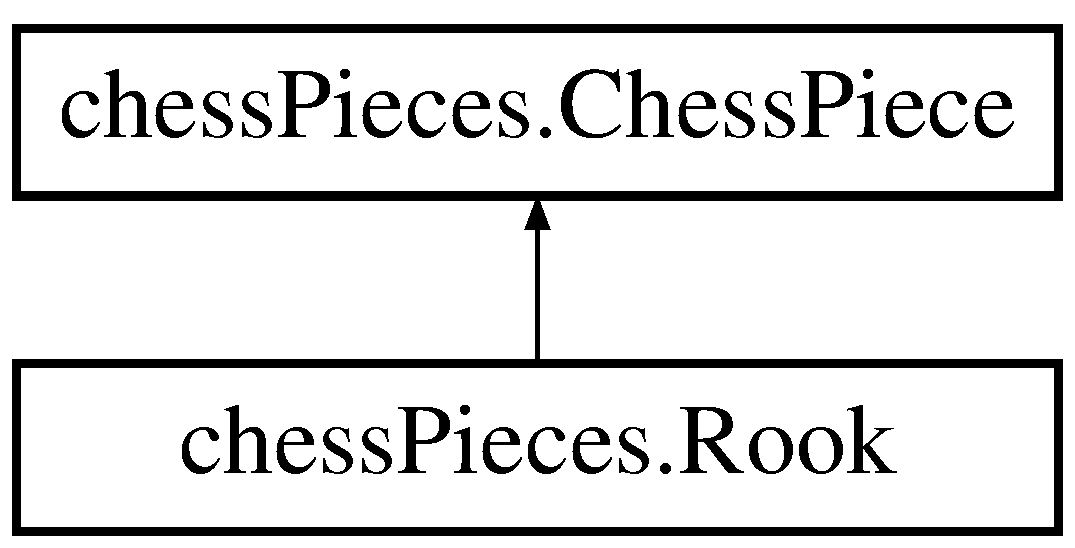
\includegraphics[height=2.000000cm]{classchess_pieces_1_1_rook}
\end{center}
\end{figure}
\subsection*{Public Member Functions}
\begin{DoxyCompactItemize}
\item 
\hyperlink{classchess_pieces_1_1_rook_a6f70e418c517ef9042b4d5f55ced440d}{Rook} (String type, int number)
\item 
\hyperlink{classchess_pieces_1_1_rook_abf88a6f46fee569655f05f56ed50631a}{Rook} (String type, \hyperlink{classmodels_1_1_position}{Position} position, int number)
\item 
\hypertarget{classchess_pieces_1_1_rook_a181f0cc6c985dd7c11689a62ebb63282}{void {\bfseries get\+Possible\+Next\+Position} (\hyperlink{classmodels_1_1_chess_board}{Chess\+Board} chess\+Board)}\label{classchess_pieces_1_1_rook_a181f0cc6c985dd7c11689a62ebb63282}

\end{DoxyCompactItemize}
\subsection*{Additional Inherited Members}


\subsection{Detailed Description}
This is the class for rook \begin{DoxyAuthor}{Author}
haoranyu 
\end{DoxyAuthor}
\begin{DoxySince}{Since}
2015-\/02-\/13 01\+:19\+:42 
\end{DoxySince}
\begin{DoxyVersion}{Version}
1.\+0 
\end{DoxyVersion}


\subsection{Constructor \& Destructor Documentation}
\hypertarget{classchess_pieces_1_1_rook_a6f70e418c517ef9042b4d5f55ced440d}{\index{chess\+Pieces\+::\+Rook@{chess\+Pieces\+::\+Rook}!Rook@{Rook}}
\index{Rook@{Rook}!chess\+Pieces\+::\+Rook@{chess\+Pieces\+::\+Rook}}
\subsubsection[{Rook}]{\setlength{\rightskip}{0pt plus 5cm}chess\+Pieces.\+Rook.\+Rook (
\begin{DoxyParamCaption}
\item[{String}]{type, }
\item[{int}]{number}
\end{DoxyParamCaption}
)}}\label{classchess_pieces_1_1_rook_a6f70e418c517ef9042b4d5f55ced440d}
Constructor for default \hyperlink{classchess_pieces_1_1_rook}{Rook}


\begin{DoxyParams}{Parameters}
{\em type} & the color or null \\
\hline
{\em number} & the numbering of rook \\
\hline
\end{DoxyParams}
\hypertarget{classchess_pieces_1_1_rook_abf88a6f46fee569655f05f56ed50631a}{\index{chess\+Pieces\+::\+Rook@{chess\+Pieces\+::\+Rook}!Rook@{Rook}}
\index{Rook@{Rook}!chess\+Pieces\+::\+Rook@{chess\+Pieces\+::\+Rook}}
\subsubsection[{Rook}]{\setlength{\rightskip}{0pt plus 5cm}chess\+Pieces.\+Rook.\+Rook (
\begin{DoxyParamCaption}
\item[{String}]{type, }
\item[{{\bf Position}}]{position, }
\item[{int}]{number}
\end{DoxyParamCaption}
)}}\label{classchess_pieces_1_1_rook_abf88a6f46fee569655f05f56ed50631a}
Constructor for \hyperlink{classchess_pieces_1_1_rook}{Rook} with specified position


\begin{DoxyParams}{Parameters}
{\em type} & the color or null \\
\hline
{\em position} & the position of this rook \\
\hline
{\em number} & the numbering of rook \\
\hline
\end{DoxyParams}


The documentation for this class was generated from the following file\+:\begin{DoxyCompactItemize}
\item 
src/chess\+Pieces/Rook.\+java\end{DoxyCompactItemize}

%--- End generated contents ---

% Index
\newpage
\phantomsection
\addcontentsline{toc}{chapter}{Index}
\printindex

\end{document}
